% =============================================================================
% TwinGuard: Confidential AI Inference at Scale
% IEEE Access submission version
% =============================================================================
\documentclass{ieeeaccess}

% ---- Encoding and fonts -----------------------------------------------------
\usepackage[utf8]{inputenc}
\usepackage[T1]{fontenc}

% ---- Mathematics ------------------------------------------------------------
\usepackage{amsmath}
\usepackage{amssymb}
\usepackage{amsfonts}
\usepackage{mathtools}
\usepackage{amsthm}
\newtheorem{definition}{Definition}
\newtheorem{theorem}{Theorem}
\newtheorem*{proof*}{Proof}

% ---- Graphics and color -----------------------------------------------------
\usepackage{graphicx}
\usepackage{xpatch}
% Biographies: fixed spacing between entries (the class default stretches it
% to fill the column, which leaves large gaps on the last page).
\makeatletter
\xpatchcmd{\IEEEbiography}{plus 1fil}{plus 2pt}{}{\PackageWarning{main}{bio patch failed}}
\xpatchcmd{\IEEEbiography}{\vskip \@IEEEBIOskipN}{\vskip 1.5\baselineskip}{}{\PackageWarning{main}{bio skip patch failed}}
\makeatother

% ---- Tables -----------------------------------------------------------------
\usepackage{tabularx}
\usepackage{booktabs}
\usepackage{multirow}
\usepackage{array}
\newcolumntype{L}{>{\raggedright\arraybackslash}X}
\newcolumntype{C}{>{\centering\arraybackslash}X}

% ---- Algorithms -------------------------------------------------------------
\usepackage{algorithm}
\usepackage{algpseudocode}
\algnewcommand\algorithmicinput{\textbf{Input:}}
\algnewcommand\algorithmicoutput{\textbf{Output:}}
\algnewcommand\Input{\item[\algorithmicinput]}
\algnewcommand\Output{\item[\algorithmicoutput]}

% ---- Hyperlinks and references ----------------------------------------------
\usepackage{hyperref}
\hypersetup{
  colorlinks=false,
  hidelinks,
  pdftitle={Confidential AI Inference at Scale: A TEE-Based Framework for Large Language Models in Regulated Cloud Environments, with a Trace-Driven Projection over 1.2 Million Real Requests},
  pdfauthor={Carlos Lucas Vieira Barbosa; Jose de Souza Junior; Allan Douglas Costa},
  pdfkeywords={Confidential Computing, Large Language Models, Remote Attestation, Trusted Execution Environments}
}
\usepackage{cite}
\usepackage{url}

% ---- Misc -------------------------------------------------------------------
\usepackage{microtype}

% =============================================================================
\begin{document}

\history{Date of publication xxxx 00, 0000, date of current version xxxx 00, 0000.}
\doi{10.1109/ACCESS.2026.XXXXXXX}

\title{Confidential AI Inference at Scale:\\
A TEE-Based Framework for Large Language\\
Models in Regulated Cloud Environments,\\
with a Trace-Driven Projection over\\
1.2 Million Real Requests}

\author{\uppercase{Carlos Lucas Vieira Barbosa}\authorrefmark{1},
\uppercase{Jos\'e de Souza Junior}\authorrefmark{2}, AND
\uppercase{Allan Douglas Costa}\authorrefmark{3}}

\address[1]{Federal University of Par\'a (UFPA), Bel\'em, Par\'a, Brazil
(e-mail: carlos.barbosa@itec.ufpa.br)}
\address[2]{University of Bras\'ilia (UnB), Bras\'ilia, DF, Brazil
(e-mail: jose.souza@unb.br)}
\address[3]{Federal Rural University of the Amazon (UFRA), Bel\'em, Par\'a, Brazil
(e-mail: allan.costa@ufra.edu.br)}

\tfootnote{This work was supported in part by the Funda\c{c}\~ao Amaz\^onia de Amparo a Estudos e Pesquisas do Par\'{a} (FAPESPA), PRODEPA, and SEC365 Cybersecurity Solutions.}

\corresp{Corresponding author: Carlos Lucas Vieira Barbosa
(e-mail: carlos.barbosa@itec.ufpa.br). ORCID: 0009-0007-7839-0749.}

\markboth{Barbosa \headeretal: TwinGuard}{Barbosa \headeretal: TwinGuard}

\begin{abstract}
As Large Language Models (LLMs) enter regulated sectors, running them in the
cloud risks exposing sensitive data. Previous research has tackled Trusted
Execution Environment (TEE) attestation, privacy, auditing, and performance
separately, lacking a unified way to compare deployments. To bridge this gap,
we introduce TwinGuard, a framework for confidential LLM inference on TEEs.
TwinGuard integrates hardware-backed attestation, encrypted-memory inference,
output perturbation, and a tamper-evident audit log mapped to General Data
Protection Regulation (GDPR) and Health Insurance Portability and
Accountability Act (HIPAA) controls. To effectively evaluate these setups, we
also introduce the Confidential Inference Score (CIS), a composite metric
designed to benchmark security and performance. We ran 1.2 million real
inference requests (Llama-2-7B on vLLM) on an NVIDIA RTX 5090 without TEE
protection, with a mean latency of 1,131.5\,ms and 14.12 requests/s. Using
these traces and Monte Carlo simulations with literature-based TEE overheads,
we projected deployments across Intel Trust Domain Extensions (TDX), AMD
Secure Encrypted Virtualization--Secure Nested Paging (SEV-SNP), and Intel
Software Guard Extensions (SGX). Projected mean latencies were 1,201\,ms (SGX),
1,231\,ms (TDX), and 1,242\,ms (SEV-SNP), with freshness-aware attestation
adding just 0.66\%. Projected CIS values reached 0.928, 0.921, and 0.918,
compared to 0.288 for Transport Layer Security (TLS)-only. SGX ranked first in
74\% of simulations, and all backends delivered 93.8\% design-level control
coverage, exceeding the 25.0\% of TLS alone. These results are trace-driven
projections rather than measurements on TEE hardware.
\end{abstract}

\begin{keywords}
Auditing, Cloud computing security, Computer security, Data privacy,
Differential privacy, Large language models, Regulation compliance, Trusted computing
\end{keywords}

\maketitle

% =============================================================================
\section{Introduction}
\label{sec:intro}
% =============================================================================

Large language models (LLMs) now process protected health information in
clinical decision support, transaction records in fraud detection, and
privileged attorney-client communications in legal assistants. Most of these
systems call cloud inference endpoints, where the cloud service provider (CSP)
can read prompts and responses in plaintext. That exposure conflicts with the
European General Data Protection Regulation (GDPR) \cite{gdpr2016}, the
Health Insurance Portability and Accountability Act (HIPAA) Security Rule
\cite{hipaa1996}, and the Payment Card Industry Data Security Standard
(PCI-DSS) \cite{pcidss2022}.

Recent work further shows that black-box production LLM APIs can expose
nontrivial model information to extraction attacks \cite{carlini2024stealing}.
Encryption at rest and in transit, such as Transport Layer Security (TLS), does not cover this case; the data must
also be protected while in use.

Trusted Execution Environments (TEEs), including Intel Software Guard
Extensions (SGX) \cite{mckeen2013innovative}, Intel Trust Domain Extensions
(TDX) \cite{inteltdx2023}, AMD Secure Encrypted Virtualization-Secure Nested
Paging (SEV-SNP) \cite{amdsev2020}, and ARM Confidential Compute Architecture
(CCA) \cite{armcca2022}, isolate computation from privileged software,
including the hypervisor and the host operating system. Running
production-scale LLMs inside these boundaries raises four open problems: (i) TEE memory
capacity constraints conflict with the multi-gigabyte activation footprint of
contemporary LLMs \cite{tramer2019slalom}; (ii) remote attestation
protocols must be integrated into the inference request path without
prohibitive latency penalties \cite{anati2013innovative}; (iii) compliance
auditing requires tamper-evident logging that is protected from
CSP observation; and (iv) no standard metric exists for quantifying the joint
privacy, attestation freshness, overhead, and selected technical-control
coverage of a confidential inference deployment.

Figure~\ref{fig:graphical-abstract} shows the workflow. The client encrypts the sensitive query before it enters the cloud;
the untrusted infrastructure can route ciphertext but should not see the
plaintext. In the proposed workflow, the TEE layer decrypts and processes the
request, optionally applies a bounded output perturbation, and protects the
response before its return. Attestation and the append-only audit structure
provide corresponding trust and traceability functions without storing sensitive text.

\subsection{Research Gap}

Existing work on private inference \cite{juvekar2018gazelle,
rathee2020cryptflow2, dong2023ciphergpt, akimoto2023privformer} relies
primarily on cryptographic protocols such as secure multiparty computation
(SMPC) and homomorphic encryption (HE). Although cryptographically rigorous,
these approaches remain orders of magnitude slower than plaintext inference
for transformer models \cite{hao2022iron}, which makes them difficult to use for
interactive deployment. TEE-based approaches
\cite{mo2021ppfl, tramer2019slalom} have demonstrated the feasibility of protected ML workloads, but have not addressed the composite challenge of attestation chain management, differential privacy
integration, compliance log integrity, and hardware-agnostic portability.
Because existing systems use different threat models, hardware, workloads,
and metrics, their results cannot be directly compared. TwinGuard combines
these functions in one multi-backend design and compares configurations with a
single composite metric, evaluated against a physical benchmark.

Table~\ref{tab:nomenclature} summarizes the principal abbreviations used
throughout the article. CIS denotes the \emph{Confidential Inference Score}
defined in Section~\ref{subsec:cis}.

\begin{table*}[t]
\caption{Core nomenclature and abbreviations used in TwinGuard.}
\label{tab:nomenclature}
\centering
\footnotesize
\setlength{\tabcolsep}{3pt}
\renewcommand{\arraystretch}{1.08}
\begin{tabular}{@{}
  >{\centering\arraybackslash\bfseries}p{0.105\textwidth}
  >{\raggedright\arraybackslash}p{0.365\textwidth}
  >{\centering\arraybackslash\bfseries}p{0.105\textwidth}
  >{\raggedright\arraybackslash}p{0.365\textwidth}@{}}
\toprule
\textbf{Term} & \textbf{Meaning in this article} &
\textbf{Term} & \textbf{Meaning in this article} \\
\midrule
CIS & Confidential Inference Score (TwinGuard composite metric) &
TEE & Trusted Execution Environment \\
LLM & Large Language Model &
CSP & Cloud Service Provider \\
TDX & Intel Trust Domain Extensions &
SGX & Intel Software Guard Extensions \\
SEV-SNP & AMD Secure Encrypted Virtualization--Secure Nested Paging &
CCA & ARM Confidential Compute Architecture \\
AA & Attestation Agent &
IA & Inference Agent \\
AUA & Audit Agent &
DP & Differential Privacy \\
PG & Privacy-related sub-score &
AF & Attestation Freshness sub-score \\
OP & Overhead Penalty sub-score &
CS & Technical-Control Coverage sub-score \\
DCAP & Data Center Attestation Primitives &
AMD-SP & AMD Secure Processor \\
KDS & AMD Key Distribution Service &
VCEK & Versioned Chip Endorsement Key \\
HKDF & HMAC-based Extract-and-Expand Key Derivation Function &
MEE & Memory Encryption Engine \\
EPC & Enclave Page Cache &
TLS & Transport Layer Security \\
GDPR & General Data Protection Regulation &
HIPAA & Health Insurance Portability and Accountability Act \\
NIST CSF & National Institute of Standards and Technology Cybersecurity Framework &
PCI-DSS & Payment Card Industry Data Security Standard \\
SMPC & Secure Multiparty Computation &
FHE & Fully Homomorphic Encryption \\
MITRE ATT\&CK & Adversarial Tactics, Techniques, and Common Knowledge &
ISO/IEC 27001 & Information security management standard \\
\bottomrule
\end{tabular}
\end{table*}

\subsection{Contributions}

This paper makes the following contributions:

\begin{enumerate}

\item \textbf{TwinGuard Framework.} A three-layer, hardware-agnostic
architecture for confidential LLM inference, coordinating an Attestation
Agent (AA), Inference Agent (IA), and Audit Agent (AUA) within TEE
boundaries. TwinGuard's hardware abstraction layer targets Intel TDX,
AMD SEV-SNP, and Intel SGX; cross-backend portability of the LLM
serving stack is a design requirement, with physical multi-backend
validation deferred to future work (see Section~\ref{sec:disc}).

\item \textbf{Confidential Inference Score (CIS).} A composite decision
metric that combines a privacy-related component, attestation freshness, the
performance cost of protection, and selected technical-control coverage, so
that TEE backends, differential privacy budgets, and deployment configurations
can be compared on one scale.

\item \textbf{Attestation-Integrated Inference Protocol.} A request-scoped
attestation protocol that is designed to amortize the cost of Data Center Attestation Primitives (DCAP)-based verification across multiple inference calls through a freshness-aware caching
mechanism. At the measured request rate, re-attestation is needed once every
$\approx 149$ requests, so attestation adds 0.66\% to the mean latency (with
187\,ms for a full attestation and 6.2\,ms for a cached check).

\item \textbf{Tamper-Evident Compliance Ledger.} A Merkle-tree-based audit
log that records every inference operation with its associated GDPR and HIPAA
control mappings, enabling automated regulatory audit trail generation without
CSP visibility into log contents.

\item \textbf{Physical Benchmark and Trace-Driven TEE Projection.} A
benchmark of 1.2 million real inference requests on an NVIDIA RTX 5090,
released with its per-request traces, and a projection of TDX, SEV-SNP, and
SGX deployments driven by these traces and by TEE overheads measured in the
literature, with Monte Carlo propagation of their uncertainty. The projection
reports latency, throughput, attestation cost, CIS, and the probability of
each backend ranking.

\end{enumerate}

The remainder of this paper is organized as follows. Section~\ref{sec:bg}
provides background on TEE technologies and related work. Section~\ref{sec:tm}
formalizes the threat model and defines the CIS metric.
Section~\ref{sec:framework} presents the TwinGuard architecture.
Section~\ref{sec:security} provides formal security and compliance analysis.
Section~\ref{sec:eval} reports the physical benchmark and the trace-driven
TEE projection. Section~\ref{sec:disc}
discusses implications and limitations. Section~\ref{sec:conc} concludes.

\Figure[t!](topskip=0pt,midskip=0pt,botskip=0pt)[width=0.80\textwidth]
{imagens/fig1-workflow.pdf}
{Overview of the TwinGuard workflow for encrypted queries, attestation,
TEE inference, privacy protection, and audit logging.\label{fig:graphical-abstract}}

% =============================================================================
\section{Background and Related Work}
\label{sec:bg}
% =============================================================================

\subsection{Trusted Execution Environments}

A Trusted Execution Environment (TEE) is a hardware-enforced isolated
processing domain that guarantees confidentiality and integrity of code and
data against a privileged software adversary, including the hypervisor and
operating system \cite{sabt2015trusted}. Modern TEE implementations differ
in their trust boundary and granularity.

\textbf{Intel SGX} partitions the processor into a privileged enclave mode
whose memory resides in the Enclave Page Cache (EPC). On client and Xeon~E
platforms, the EPC is protected by the Memory Encryption Engine (MEE), which
provides encryption with an integrity tree; on third-generation Xeon Scalable
processors, SGX instead relies on Total Memory Encryption--Multi-Key (TME-MK) with Advanced Encryption Standard (AES)-XTS-128, which enables much larger EPCs but omits the integrity tree
\cite{elhindi2022sgx}. SGX provides remote attestation
through the Intel DCAP protocol, enabling
verifiable proof that specific code runs within a genuine Intel processor
\cite{anati2013innovative, johnson2016intel}. First-generation EPC was
limited to 128--256\,MB; third-generation Intel Xeon Scalable (Ice Lake)
processors support up to 512\,GB of EPC per socket, depending on the CPU
model \cite{elhindi2022sgx, lenovo2023sgx}, substantially reducing the paging burden for
large-model workloads. The Enclave Dynamic Memory Management (EDMM) feature of SGX2 only allows enclave pages to be
added, removed, or re-protected dynamically; it does not change EPC capacity.

\textbf{Intel TDX} \cite{inteltdx2023} extends confidential computing to the virtual machine (VM) level, creating Trust Domains (TDs) where the entire VM
memory is encrypted and integrity-protected. TDX eliminates SGX's EPC
constraint, making it suitable for workloads with large memory footprints
such as LLM inference. TDX's remote attestation is also DCAP-based but
operates at the TD Report granularity.

\textbf{AMD SEV-SNP} \cite{amdsev2020} protects VMs through memory
encryption with AES-128-XEX, integrity checking via a Reverse Map Table (RMP),
and secure nested page tables. Unlike Intel's DCAP, SEV-SNP attestation
reports are generated by the AMD Secure Processor (AMD-SP) embedded in the
CPU die and are verified through AMD's Key Distribution Service (KDS) using
the Versioned Chip Endorsement Key (VCEK) certificate chain, rooted at the
AMD Root Key (ARK) and Signing Key (ASK).

\textbf{ARM CCA} \cite{armcca2022} introduces Realms as hardware-isolated
computation domains protected against the hypervisor, complementing
TrustZone \cite{pinto2019demystifying} for cloud-scale deployment.

\subsection{TEE-Based Inference Systems}

Recent work has also evaluated confidential LLM serving on modern CPU and GPU
TEEs. Chrapek \emph{et al.} \cite{chrapek2025confidential} run full Llama~2
inference pipelines (7B, 13B, and 70B) in Intel TDX and SGX and on NVIDIA H100
confidential GPUs. For Llama-2-7B they measure overheads of 5.51--10.68\% for
TDX and 4.80--6.15\% for SGX, and throughput penalties of 4--8\% on the
confidential GPUs; we use their TDX and SGX ranges as inputs to the
projection in Section~\ref{sec:eval}. PipeLLM \cite{tan2024pipellm} reduces
the overhead of confidential-GPU LLM serving on NVIDIA H100 with speculative
pipelined encryption.

\textbf{Slalom} \cite{tramer2019slalom} partitions deep neural network (DNN) inference between an
SGX enclave and an untrusted, co-located GPU. All linear layers are delegated
to the GPU; the enclave verifies their results with Freivalds' algorithm and
can blind their inputs with precomputed pseudorandom streams, providing
integrity and, optionally, privacy. On VGG16, MobileNet, and ResNet variants,
Slalom reports $6$--$20\times$ higher throughput for verifiable inference and
$4$--$11\times$ for verifiable and private inference, compared with running
the full model inside the enclave. Its evaluation covers convolutional
networks only, and its precomputed blinding factors assume fixed weights and
known layer shapes, which has not been demonstrated for autoregressive LLMs.
TwinGuard instead keeps the model inside an attested trust boundary and
avoids per-layer verification.

\textbf{PPFL} \cite{mo2021ppfl} uses TEEs on both sides of federated learning:
Arm TrustZone on the clients for local training and Intel SGX on the server
for secure aggregation, so that model and gradient updates remain hidden.
To fit the limited TEE memory, it trains the model greedily one layer at a
time and reports protection against data reconstruction, property inference,
and membership inference attacks, with up to about 15\% CPU-time overhead on
the client. PPFL targets privacy during federated training rather than
inference-time protection of user queries, and does not address regulatory
control mapping. Because the threat models, workloads, and evaluation
settings of these systems differ from confidential LLM inference, we compare
TwinGuard with them qualitatively.

\subsection{Cryptographic Private Inference}

\textbf{GAZELLE} \cite{juvekar2018gazelle} combines homomorphic encryption for
linear layers with garbled circuits for non-linear activations and reports an
end-to-end latency of 30\,ms for an MNIST network and 3.6\,s for a CIFAR-10
network in a local area network (LAN) setting. \textbf{CrypTFlow2} \cite{rathee2020cryptflow2}
replaces garbled circuits with new protocols based on oblivious transfer (OT) for
ReLU and truncation, and is the first to run ImageNet-scale networks such as
ResNet50 and DenseNet121 securely. Both target convolutional networks; neither
evaluates transformers.

\textbf{IRON} \cite{hao2022iron} brings two-party private inference to
transformers. It uses a Brakerski--Fan--Vercauteren (BFV)-based homomorphic
matrix-multiplication protocol
and secret-sharing and oblivious-transfer protocols for Softmax, GELU, and
LayerNorm, and evaluates BERT models from BERT-Tiny to BERT-Large. It reports
3--11$\times$ less runtime than the prior state of the art, but end-to-end
runtimes remain in the range of minutes per inference.
\textbf{CipherGPT} \cite{dong2023ciphergpt} extends two-party private
inference to GPT-style models, with protocols for matrix multiplication, GELU,
and top-$k$ sampling. \textbf{PrivFormer} \cite{akimoto2023privformer}
follows a different setting: a three-party, honest-majority SMPC protocol
that approximates attention with ReLU-based kernels and requires
non-colluding computation parties.

These systems provide strong guarantees without trusting hardware, but their
interactive protocols cost orders of magnitude more than plaintext inference,
and none addresses attestation, audit logging, or regulatory control mapping.
Because their workloads, models, and evaluation settings differ from ours,
we compare them only qualitatively (Table~\ref{tab:related}).

\subsection{Differential Privacy for LLMs}

\textbf{Dwork et al.} \cite{dwork2014algorithmic} formalized differential privacy (DP) and the Gaussian mechanism that TwinGuard employs for logit-level
output perturbation. DP stochastic gradient descent (DP-SGD) \cite{abadi2016deep} extends DP to the training
phase via per-gradient clipping and noise addition, enabling private
fine-tuning of LLMs. While DP-SGD protects training data membership,
it does not protect query inputs at inference time, which is the threat model
TwinGuard addresses. \textbf{Yu et al.} \cite{yu2022differentially} report differentially private fine-tuning of
language models at $\epsilon \approx 6$--$7$ ($\delta = 10^{-5}$ or
$10^{-6}$) with accuracy within a few points of the non-private baseline,
indicating that DP can be compatible with useful accuracy. Song and
Raghunathan \cite{song2020information} show that embeddings leak information
about their inputs, a risk that output-level perturbation may help to reduce.
In TwinGuard, the Inference Agent can apply per-query output perturbation and
reports the privacy budget it consumes in the compliance log.

\subsection{Regulatory Compliance in Cloud AI}

\textbf{GDPR} \cite{gdpr2016} Article 25 mandates data protection by design
and by default, requiring that technical measures ensure only necessary data
is processed. Article 32 requires appropriate encryption, pseudonymization,
and ongoing confidentiality assurance. European Data Protection Board
recommendations on supplementary measures \cite{edpb2021} regard technical
measures such as encryption, where the provider has no access to plaintext, as
relevant safeguards; this motivates attestation-backed protection of data in use. Prior work \cite{gruschka2010privacy}
characterizes cloud-service attack surfaces, but does not address
hardware-level enforcement.

\textbf{HIPAA} \cite{hipaa1996} imposes analogous requirements for
electronic Protected Health Information (ePHI) under the Security Rule,
including access controls (45 CFR 164.312(a)), audit controls (164.312(b)),
integrity controls (164.312(c)), and transmission security (164.312(e)).
\textbf{Ryan} \cite{ryan2011cloud} discusses privacy concerns of cloud computing
before hardware TEEs were available, when users could only trust the CSP.
TwinGuard replaces part of that trust with attestation and hardware isolation.

\textbf{Pearson and Benameur} \cite{pearson2012privacy} survey
privacy-enhancing technologies for cloud computing, identifying audit
logging and access control as the primary compliance gaps in multi-tenant
environments. Their survey predates TEE deployment for LLMs and proposes no
quantitative compliance metric. For LLM inference, TwinGuard covers audit
logging with its Merkle-tree log and access control with attestation-bound
session tokens, and adds the CIS as a quantitative score.

\subsection{Comparative Analysis}

Table~\ref{tab:related} positions TwinGuard against the most relevant prior
work across six dimensions. None of the listed systems covers all six.

\begin{table*}[t]
\caption{Qualitative comparison of TwinGuard and related approaches across six
technical dimensions.}
\label{tab:related}
{\renewcommand{\arraystretch}{1.12}
\begin{tabularx}{\textwidth}{l L L C C C C}
\toprule
\textbf{Approach} & \textbf{TEE Backend} & \textbf{LLM Scale} &
\textbf{HW-Agnostic} & \textbf{Composite Metric} &
\textbf{Technical Map} & \textbf{Audit Log} \\
\midrule
Slalom \cite{tramer2019slalom}           & SGX + GPU        & Convolutional neural network & No  & No  & No  & No  \\
PPFL \cite{mo2021ppfl}                  & SGX + TrustZone  & FL training  & No  & No  & No  & No  \\
CipherGPT \cite{dong2023ciphergpt}      & Two-party SMPC (no TEE) & GPT-2    & N/A & No  & No  & No  \\
PrivFormer \cite{akimoto2023privformer} & Three-party SMPC (no TEE) & Transformer   & N/A & No  & No  & No  \\
IRON \cite{hao2022iron}                 & Two-party HE/OT (no TEE) & BERT  & N/A & No  & No  & No  \\
Chrapek \emph{et al.} \cite{chrapek2025confidential} & TDX, SGX, cGPU & Llama 2 (7--70B) & No & No & No & No \\
PipeLLM \cite{tan2024pipellm}           & NVIDIA cGPU      & 13--175B & No & No & No & No \\
\midrule
\textbf{TwinGuard (ours)}               & \textbf{SGX, TDX, SEV-SNP} & \textbf{7--70B (design)} &
\textbf{By design} & \textbf{Yes (CIS)} & \textbf{Yes} & \textbf{Yes} \\
\bottomrule
\end{tabularx}
}
\end{table*}

% =============================================================================
\section{Threat Model and Problem Formulation}
\label{sec:tm}
% =============================================================================

\subsection{System Model}

We consider a three-party system: a \emph{Client} $\mathcal{C}$ who holds
sensitive query data $x$, a \emph{Cloud Service Provider} $\mathcal{P}$ who
operates the compute infrastructure and LLM model $\mathcal{M}$, and a
\emph{Regulator} $\mathcal{R}$ who requires evidence of compliance with
privacy mandates. TwinGuard is deployed on $\mathcal{P}$'s infrastructure
within TEE-protected enclaves.

\subsection{Adversary Model}

We model a probabilistic polynomial-time (PPT) adversary $\mathcal{A}$ with the
following capabilities:

\textbf{Honest-but-curious CSP.} $\mathcal{P}$ executes the protocol
faithfully but attempts to learn $x$ or model outputs by observing all
software-accessible memory, I/O channels, and system logs.

\textbf{Malicious insider.} A system administrator with root privileges
on the host OS and hypervisor attempts to extract enclave memory or intercept
network traffic.

\textbf{Network adversary.} An adversary $\mathcal{A}_{\text{net}}$ with
full control over the network between $\mathcal{C}$ and $\mathcal{P}$
(Dolev-Yao model \cite{dolev1983security}) attempts to intercept, modify,
or replay inference requests and responses.

\textbf{Physical attacker.} An adversary $\mathcal{A}_{\text{phys}}$ with
physical access to the server, capable of cold-boot attacks, DRAM probing,
and PCIe bus snooping. We consider physical CPU package attacks to be
out-of-scope, as they require defeating hardware root-of-trust.
The reference configuration uses the RTX 5090 as an inference accelerator.
The protection considered in this study focuses on the CPU environment, while
confidential mechanisms for GPU memory and interconnect represent a natural
extension for future deployments.

\subsection{Conditional Security Goals}

The TwinGuard framework is evaluated against the following conditional
security goals. Each goal is framed by the cryptographic, hardware, and
trust-boundary conditions defined in this work:

\begin{itemize}
\item \textbf{P1 (Data Confidentiality Goal).} For all PPT $\mathcal{A}$, the probability
of distinguishing two input queries $x_0$ and $x_1$ given only the
observations available to an honest-but-curious CSP is
$\Pr[\mathcal{A} \text{ wins}] \leq \frac{1}{2} + \mathsf{negl}(\lambda)$,
where $\lambda$ is the security parameter.

\item \textbf{P2 (Model Privacy Goal).} Outside the TEE, the weights $\theta$ of
$\mathcal{M}$ exist only as authenticated ciphertexts, so that a PPT
$\mathcal{A}$ learns nothing about $\theta$ beyond its size except with
probability $\mathsf{negl}(\lambda)$.

\item \textbf{P3 (Inference Integrity Goal).} For all valid requests $x$, the
probability that $\mathcal{A}$ causes $\mathcal{M}(x)$ to return a value
$y' \neq \mathcal{M}(x)$ without detection is $\mathsf{negl}(\lambda)$.

\item \textbf{P4 (Audit Integrity Goal).} The audit log $\mathcal{L}$ is
collision-resistant: no PPT adversary can produce entries
$(e_1, e_2)$ such that $\mathcal{H}(e_1) = \mathcal{H}(e_2)$ but
$e_1 \neq e_2$, where $\mathcal{H}$ is the Merkle hash function.

\item \textbf{P5 (Attestation Soundness Goal).} The probability that a forged
attestation report is accepted as genuine is $\mathsf{negl}(\lambda)$ assuming that the hardware root of trust is not compromised.
\end{itemize}

\subsection{Definition: Confidential Inference Score}
\label{subsec:cis}

We introduce the \emph{Confidential Inference Score} (CIS), a composite
metric in $[0,1]$ that scores the protection of a deployment for each
inference request. Let $\mathcal{I} = \{q_1, q_2, \ldots, q_n\}$ be
a sequence of inference requests processed by TwinGuard.

\begin{definition}[Confidential Inference Score]
\label{def:cis}
For inference request $q_i$, the Confidential Inference Score is:
\begin{equation}
\label{eq:cis}
\mathrm{CIS}(q_i) = \alpha \cdot \mathrm{PG}(q_i)
                  + \beta  \cdot \mathrm{AF}(q_i)
                  + \gamma \cdot (1 - \mathrm{OP}(q_i))
                  + \delta \cdot \mathrm{CS}(q_i),
\end{equation}
where the weight vector $(\alpha, \beta, \gamma, \delta) = (0.35, 0.25, 0.25, 0.15)$
satisfies $\alpha + \beta + \gamma + \delta = 1$, and the four sub-scores are
defined as follows.
\end{definition}

\textbf{Privacy-related score} $\mathrm{PG}(q_i) \in [0,1]$ is an
exploratory score for the configured output-perturbation setting:
\begin{equation}
\label{eq:pg}
\mathrm{PG}(q_i) = \left(1 - \frac{\epsilon(q_i)}{\epsilon_{\max}}\right)
                   \cdot \mathbf{1}[\text{MEE}(q_i) \geq \text{AES-128}],
\end{equation}
where $\epsilon(q_i)$ is the configured perturbation parameter,
$\epsilon_{\max}$ is a policy-selected normalization constant, and
$\mathbb{1}[\cdot]$ indicates that memory encryption of at least
AES-128 strength is active.

\textbf{Attestation Freshness} $\mathrm{AF}(q_i) \in [0,1]$ models the
decay of trust in the attestation report as time since last attestation
increases:
\begin{equation}
\label{eq:af}
\mathrm{AF}(q_i) = e^{-\lambda_a \cdot \Delta t(q_i)},
\end{equation}
where $\Delta t(q_i) = t_i - t_{\text{att}}$ is the elapsed time since the
last successful attestation for the enclave serving $q_i$, and
$\lambda_a$ is the freshness decay rate (default $\lambda_a = 0.01\,\mathrm{s^{-1}}$, configurable per policy).

\textbf{Overhead Penalty} $\mathrm{OP}(q_i) \in [0,1]$ captures the
normalized latency cost introduced by TEE protection:
\begin{equation}
\label{eq:op}
\mathrm{OP}(q_i) = \min\!\left(1,\ \frac{L_{\mathrm{TEE}}(q_i) -
L_{\mathrm{base}}(q_i)}{L_{\mathrm{base}}(q_i)}\right),
\end{equation}
where $L_{\mathrm{TEE}}$ and $L_{\mathrm{base}}$ are inference latencies
with and without TEE protection, respectively.

\textbf{Technical-Control Coverage} $\mathrm{CS}(q_i) \in [0,1]$ measures the
fraction of selected, applicable technical controls represented as satisfied
for $q_i$:
\begin{equation}
\label{eq:cs}
\mathrm{CS}(q_i) = \frac{|\mathcal{S}(q_i)|}{|\mathcal{R}(q_i)|},
\end{equation}
where $\mathcal{R}(q_i)$ is the set of selected controls associated with
GDPR, HIPAA, or both, depending on the client configuration, and
$\mathcal{S}(q_i) \subseteq \mathcal{R}(q_i)$ is the set of satisfied
controls under the study's mapping, as recorded by the Audit Agent.

The aggregate CIS over a deployment is defined as:
\begin{equation}
\label{eq:cis-agg}
\overline{\mathrm{CIS}} = \frac{1}{n} \sum_{i=1}^{n} \mathrm{CIS}(q_i).
\end{equation}

\textbf{Interpretation.} $\mathrm{CIS} = 1.0$ represents the theoretical
ideal: peak privacy-centric protection, a freshly attested enclave, zero
overhead, and complete coverage under the selected mapping. We use
$0.90$ as an \emph{illustrative policy threshold}. For reference, a deployment
with $\mathrm{AF}\ge 0.90$, $\mathrm{PG}\ge 0.90$, $\mathrm{OP}\le 0.15$, and
coverage $\mathrm{CS}$ satisfies
\begin{multline}
\label{eq:threshold}
\mathrm{CIS} \ge 0.35(0.90) + 0.25(0.90) \\
+ 0.25(0.85) + 0.15\,\mathrm{CS},
\end{multline}
\noindent which is equal to $0.9025$ for full coverage ($\mathrm{CS}=1$) and
$0.893$ for the design-level coverage of TwinGuard ($\mathrm{CS}=7.5/8$,
Table~\ref{tab:compliance}). A deployment at the edge of these conditions can
therefore fall slightly below $0.90$; therefore, we treat the threshold as a policy setting. Values below $0.70$ indicate a low score under the selected
technical criteria.

% =============================================================================
\section{The TwinGuard Framework}
\label{sec:framework}
% =============================================================================

\subsection{Architecture Overview}

TwinGuard organizes confidential LLM inference into three functional layers,
each corresponding to one autonomous agent, as depicted in
Fig.~\ref{fig:arch}.

% Corrected monochrome PDF for the published Figure 2 architecture diagram.
\Figure[t!](topskip=0pt,midskip=0pt,botskip=0pt)[width=0.72\textwidth]
{imagens/fig2-architecture.png}
{Logical TwinGuard architecture with the application programming interface (API) gateway, Attestation, Inference,
and Audit Agents. TDX, SEV-SNP, and SGX are alternative TEE backends.\label{fig:arch}}
% ---- External access --------------------------------------------------------


The \textbf{Attestation Agent (AA)} is TwinGuard's trust anchor. Before
any inference request is processed, the AA establishes a verified proof that the inference enclave runs the authentic TwinGuard code on genuine TEE hardware.
AA maintains a freshness-aware token cache that amortizes attestation costs across multiple client sessions.

The \textbf{Inference Agent (IA)} executes the LLM forward pass within the
TEE boundary. The IA receives decrypted inputs, performs inference using an
encrypted-in-memory model copy, applies the configured differential privacy
mechanism to outputs, re-encrypts results, and emits a structured event record
to the Audit Agent.

The \textbf{Audit Agent (AUA)} maintains a tamper-evident Merkle-tree audit
log of all inference events, enriched with GDPR and HIPAA control mappings.
AUA runs in a protection domain separate from IA so that a compromised IA
cannot forge audit entries: a separate enclave on SGX, a separate trust domain
on TDX, or a separate VM privilege level (VMPL) on SEV-SNP.

\subsection{Inter-Agent Protocol and Sequence Flow}

The end-to-end protocol is illustrated in Fig.~\ref{fig:seq}. The protocol proceeds in four phases: initialization, attestation, inference, and auditing.

\Figure[t!](topskip=0pt,midskip=0pt,botskip=0pt)
[width=\textwidth]
{imagens/fig3-sequence.pdf}
{Modeled interaction sequence among TwinGuard agents. Line styles denote
attestation, inference, audit, and error messages; evidence follows the selected
backend.\label{fig:seq}}


\subsection{Attestation Agent: Design and Protocol}

The Attestation Agent implements a freshness-aware token cache to amortize
the high cost of full DCAP attestation. The caching policy is governed by
the Attestation Freshness score $\mathrm{AF}(q_i)$ defined in
Eq.~(\ref{eq:af}). When $\mathrm{AF}(q_i) < \theta_{\text{att}}$ (default $\theta_{\text{att}} = 0.90$), full re-attestation is triggered; otherwise,
the cached token is refreshed with a lightweight nonce.

AA generates attestation reports using the hardware-specific attestation
library for each TEE backend: for Intel TDX, the TDX DCAP Quoting Library
produces a TD Quote signed by the Intel Provisioning Certification Enclave
\cite{inteltdx2023}; for Intel SGX, the SGX DCAP Quote Generation Library
produces an Enclave Quote over MRENCLAVE \cite{johnson2016intel}; for
AMD SEV-SNP, the AMD-SP generates an Attestation Report signed with VCEK
and verifiable through AMD's KDS certificate chain \cite{amdsev2020} ---
a distinct attestation path that does not use Intel DCAP. In all cases,
the signed report covers a backend-specific measurement (MRENCLAVE for SGX,
TD measurement/RTMR values for TDX, and a VM measurement for SEV-SNP), which
the client verifies against the respective
hardware vendor's root certificate chain.

\subsection{Inference Agent: Memory Architecture}

The Inference Agent manages model weights using a chunk-based encryption
scheme. The LLM's parameter tensor is partitioned into fixed-size chunks
$\mathcal{K} = \{c_1, c_2, \ldots, c_K\}$. Each chunk $c_k$ is encrypted with AES-256 in Galois/Counter Mode (GCM) under a per-chunk key $k_c$ derived via the hash-based message authentication code (HMAC)-based Extract-and-Expand Key Derivation Function (HKDF) from the
master key $k_m$ sealed to the enclave identity:
$k_c = \mathrm{HKDF}(k_m \| \mathrm{idx}(c_k) \| \mathrm{nonce})$,
with chunk size $S_c = 256$\,MB (configurable). During forward pass, only the
active layer's chunks are decrypted into
protected enclave memory, minimizing the plaintext memory footprint.
This design reduces the effective EPC pressure for SGX deployments while
maintaining full encryption for TDX and SEV-SNP.

Differential privacy is applied as \emph{logit-level output perturbation}.
Prior to token sampling, the pre-softmax logit tensor
$y \!=\! \mathcal{M}(x) \!\in\! \mathbb{R}^{|\mathcal{V}|}$ is perturbed
with Gaussian noise $\mathcal{N}(0, \sigma^2 \mathbf{I})$, where
$\sigma \!=\! \Delta_f \sqrt{2 \ln(1.25/\delta_{\mathrm{dp}})} / \epsilon$
where $\delta_{\mathrm{dp}}$ is the DP failure probability (distinct from the CIS weight $\delta$) and $\Delta_f$ is the $\ell_2$-sensitivity of the final linear layer
\cite{dwork2014algorithmic}. Logit-level perturbation is the standard
approach for LLM output DP: operating in a continuous space preserves the
Gaussian mechanism's formal guarantees; discrete post-sampling outputs
would instead require the exponential mechanism \cite{mcsherry2007mechanism}.
Per-query $\epsilon$ is tracked by the IA and forwarded to the AUA for
the compliance log.

\subsection{Audit Agent: Tamper-Evident Ledger}

The Audit Agent maintains a Merkle tree over all inference events. Each
leaf node $\ell_i$ stores a Secure Hash Algorithm (SHA-256) hash of the inference event record:
$\ell_i = \mathrm{SHA\text{-}256}(q_i \| t_i \| \mathrm{CIS}(q_i) \| \text{ctrl\_map}(q_i))$,
where $\text{ctrl\_map}(q_i)$ is a compact bitfield indicating which
GDPR and HIPAA controls are satisfied for $q_i$. The Merkle root $r$ is
periodically signed by the enclave's sealing key and published to the
client, enabling efficient inclusion proofs for regulatory auditors.

\subsection{Main Algorithm and Complexity Analysis}

Algorithm~\ref{alg:main} presents the TwinGuard inference protocol, with the
CIS computation highlighted.

\begin{algorithm}[t]
\caption{TwinGuard Confidential Inference Protocol}
\label{alg:main}
\footnotesize
\begin{algorithmic}[1]
\Input{$q_i$: inference request; $K_s$: session key; $\tau$: attestation token;
$(\epsilon,\delta_{\mathrm{dp}})$: DP parameters; $\epsilon_{\max}$: normalization
constant; $\lambda_a,\theta_{\text{att}}$: freshness decay and threshold;
$t_{\text{att}}$: last attestation time; $L_{\mathrm{base}}$: baseline latency;
$\mathbf{w}=(\alpha,\beta,\gamma,\delta)$: CIS weights; $\Delta_f$: sensitivity}
\Output{$\mathrm{Enc}_{K_s}(y_\epsilon)$, $\mathrm{CIS}(q_i)$, Merkle root $r$}
\Statex
\Statex \textbf{Attestation Agent (AA):}
\State $\mathrm{AF} \gets e^{-\lambda_a \cdot (t_{\text{now}} - t_{\text{att}})}$
\If{$\mathrm{AF} < \theta_{\text{att}}$}
\State $\tau \gets \text{Backend.Attest}(\text{measurement},\text{nonce})$
  \State $t_{\text{att}} \gets t_{\text{now}}$; update cache
\EndIf
\State Send $\tau$; verify client acknowledgment
\Statex
\Statex \textbf{Inference Agent (IA):}
\State $x \gets \mathrm{Dec}_{K_s}(q_i.\mathrm{payload})$
\State Load active-layer chunks $\{c_k\}$ into protected memory
\State $y \gets \mathcal{M}(x)$  \Comment{LLM pass in enclave}
\State $\sigma \gets \Delta_f \sqrt{2\ln(1.25/\delta_{\mathrm{dp}})} / \epsilon$
\State $y_\epsilon \gets y + \mathcal{N}(\mathbf{0},\, \sigma^2 \mathbf{I})$
\State $\mathrm{OP} \gets \min(1,\, (L_\text{TEE} - L_\text{base}) / L_\text{base})$
\Statex
\Statex \textbf{CIS Computation:}
\State $\mathrm{PG} \gets (1-\epsilon/\epsilon_{\max})\,\mathbf{1}[\mathrm{MEE}\geq\mathrm{AES\text{-}128}]$
\State $\mathrm{CS} \gets |\mathcal{S}(q_i)|/|\mathcal{R}(q_i)|$
\State $\mathrm{CIS}(q_i) \gets \alpha\,\mathrm{PG}+\beta\,\mathrm{AF}+\gamma(1-\mathrm{OP})+\delta\,\mathrm{CS}$
\Statex
\Statex \textbf{Audit Agent (AUA):}
\State $\ell_i \gets \mathrm{SHA\text{-}256}(q_i\|t_i\|\mathrm{CIS}(q_i)\|\mathrm{ctrl\_map}(q_i))$
\State $r \gets \text{MerkleTree.Append}(\ell_i)$
\State \Return $\mathrm{Enc}_{K_s}(y_\epsilon)$, $\mathrm{CIS}(q_i)$, $r$
\Statex
\Statex \textbf{Complexity:} $O(N_\ell \cdot d^2)$ per request ($N_\ell$ layers, width $d$); $O(\log n)$ per audit append.
\end{algorithmic}
\end{algorithm}

% Let the next section fill the remaining column after the algorithm float.

% =============================================================================
\section{Security Analysis and Compliance}
\label{sec:security}
% =============================================================================

\subsection{Conditional Security Arguments}

The following arguments outline how the proposed mechanisms address the
security goals under explicit cryptographic and hardware conditions. Their
applicability is limited to the stated design; deployment-level evaluation of
physical confidentiality, side-channel resistance, GPU memory protection, and
attestation remains a subsequent evaluation stage.

\begin{itemize}
\item \textbf{P1 (Data Confidentiality).} Client inputs are encrypted under
session key $K_s$ (256-bit AES-GCM) before leaving the client, and decrypted
only within the TEE boundary where the host OS has no plaintext access.
The confidentiality of $K_s$ follows from the security of the elliptic-curve Diffie--Hellman (ECDH) key agreement executed during attestation, which is computational
indistinguishable under the decisional Diffie--Hellman (DDH) assumption
\cite{boneh1998decision}.
The TEE memory encryption (MEE or TME-MK AES-XTS-128 for SGX, AES-XTS-128
TME-MK for TDX, and AES-128 for SEV-SNP) protects memory contents in DRAM. Under these
conditions, the construction provides a basis for the P1 confidentiality goal:
$\Pr[\mathcal{A} \text{ wins P1}] \leq \frac{1}{2} + \mathsf{negl}(\lambda)$.

\item \textbf{P2 (Model Privacy).} Model weights $\theta$ are encrypted under
per-chunk keys derived from $k_m$, which is sealed to the enclave
measurement and inaccessible to the host. HKDF is a secure key
derivation function under the assumption that HMAC is a pseudorandom function
\cite{krawczyk2010cryptographic}, so the derived keys $\{k_c\}$ are
indistinguishable from independent random keys. The confidentiality of each
chunk then reduces to indistinguishability under chosen-plaintext attack
(IND-CPA) security of AES-256-GCM. This analysis provides a basis
for the intended P2 model-privacy goal.

\item \textbf{P3 (Inference Integrity).} AES-GCM authenticates each response
over $(y_\epsilon, \mathrm{CIS}(q_i), t_i)$. Under the ciphertext-integrity
(INT-CTXT) security of AES-GCM \cite{bellare2008foundations} with 128-bit tags, ciphertext
tampering is detected except with negligible probability. The Merkle proof binds $y_\epsilon$ to its audit event.

\item \textbf{P4 (Audit Integrity).} The Merkle tree uses SHA-256, which is
assumed to be collision resistant; no random-oracle assumption is required.
Replacing or inserting a leaf without changing the signed root requires a
SHA-256 collision or second preimage. By the birthday bound, an adversary
evaluating the hash $q$ times finds a collision with probability at most
about $q^2/2^{257}$. Together,
these properties contribute to the P4 audit-integrity goal against
collision-based forgery.

\item \textbf{P5 (Attestation Soundness).} The DCAP attestation chain terminates
at the hardware vendor's root certificate (Intel Root CA or AMD ARK).
Forging an attestation quote requires either compromising the CPU fuse key
or breaking the RSA-3072 or elliptic curve digital signature algorithm (ECDSA) P-384 signatures on the certificate chain,
both of which are computationally infeasible under standard assumptions
\cite{johnson2016intel, amdsev2020}. This reasoning underpins the P5
attestation-soundness goal when the hardware root of trust remains intact.
\end{itemize}

\subsection{Output Perturbation Mechanism and Intended Privacy Properties}

TwinGuard applies Gaussian logit perturbation as a configurable
privacy--utility mechanism. A formal $(\epsilon,\delta)$-differential privacy
claim would require a defined adjacency relation, bounded sensitivity,
composition accounting, and a validated implementation. These prerequisites
are outside the scope of the present study; the mechanism is therefore
reported as an intended privacy-enhancing design element rather than a formal
DP guarantee.

The perturbation does not contribute to P1. The CSP is excluded from the
plaintext by encryption and TEE isolation, not by noise. Its role is
different: it limits what the \emph{recipients} of the outputs can infer about
the model or about data reflected in it, for example through model-extraction
or membership-inference queries over the authorized interface
\cite{carlini2024stealing}. Because noise is added to the logits of every
generated token, the privacy loss composes over the response. Under basic
composition, a response of up to 128 tokens with per-token parameter
$\epsilon$ consumes up to $128\,\epsilon$. A deployment that requires a formal
guarantee must therefore apply an accountant such as R\'enyi DP
\cite{mironov2017renyi}. For these reasons, the component is optional in
TwinGuard and is not required for P1--P5.

\subsection{GDPR and HIPAA Control Mapping}

Table~\ref{tab:compliance} maps selected TwinGuard technical controls to
GDPR Articles and HIPAA Security Rule sections. The CIS technical-mapping
score $\mathrm{CS}(q_i)$ is computed deterministically from this
author-defined mapping: each control receives 1 if provided by design, 0.5 if
only partially provided, and 0 otherwise, for each regime. This mapping is not a legal compliance assessment,
certification, or independent audit.

\begin{table*}[t]
\caption{Mapping between TwinGuard technical controls and selected GDPR and
HIPAA requirements. Score: 1 = provided by design, 0.5 = partial; coverage is
the mean score over the eight controls.}
\label{tab:compliance}
{\renewcommand{\arraystretch}{1.10}
\setlength{\tabcolsep}{3.5pt}
\begin{tabularx}{\textwidth}{@{}L L L c C@{}}
\toprule
\textbf{TwinGuard Control} & \textbf{GDPR Article} & \textbf{HIPAA Section} &
\textbf{Agent} & \textbf{Score} \\
\midrule
Hardware memory encryption (AES-128/256)  & Art. 5(1)(f), Art. 32(1)(a) & 164.312(a)(2)(iv), 164.312(e)(2)(ii) & IA  & 1 \\
Remote attestation                    & Art. 25(1), Art. 32(1)(b)   & 164.308(a)(1)(ii)(B)                  & AA  & 1 \\
Configured Gaussian output perturbation & Art. 5(1)(c), Art. 25      & 164.312(a)(2)(iv), 164.308(a)(1)(ii)(B) & IA & 1 \\
Encrypted session (TLS 1.3 + AES-GCM) & Art. 32(1)(a)               & 164.312(e)(1), 164.312(e)(2)(i)       & AA  & 1 \\
Tamper-evident audit log              & Art. 5(2), Art. 32(1)(d)    & 164.312(b), 164.308(a)(1)(ii)(D)      & AUA & 1 \\
Access control (session token $\tau$) & Art. 25(2), Art. 32(1)(b)   & 164.312(a)(1)                         & AA  & 1 \\
Data minimization (query scoping)     & Art. 5(1)(c), Art. 25(1)    & 164.308(a)(3)                         & IA  & 0.5 \\
Breach detection (integrity check)    & Art. 32(1)(d), Art. 33      & 164.312(c)(1), 164.308(a)(6)          & AUA & 1 \\
\midrule
\multicolumn{4}{@{}l}{\textbf{Design-level coverage, GDPR (7.5/8 controls)}} & \textbf{93.8\%} \\
\multicolumn{4}{@{}l}{\textbf{Design-level coverage, HIPAA (7.5/8 controls)}} & \textbf{93.8\%} \\
\bottomrule
\end{tabularx}
}
\end{table*}

\subsection{NIST Cybersecurity Framework and ISO/IEC 27001 Mapping}

Table~\ref{tab:nist-iso} maps TwinGuard's technical controls to the National Institute of Standards and Technology (NIST) Cybersecurity Framework 2.0 (CSF) \cite{nistcsf2024} functions and to the International Organization for Standardization/International Electrotechnical Commission (ISO/IEC) 27001:2022 \cite{iso27001_2022} Annex~A controls, complementing the
GDPR/HIPAA mapping in Table~\ref{tab:compliance}.

\begin{table*}[t]
\caption{Mapping of TwinGuard controls to the NIST Cybersecurity Framework 2.0
and ISO/IEC 27001:2022. All controls are provided by design, except the one
marked $\dagger$, which is partial (Table~\ref{tab:compliance}).}
\label{tab:nist-iso}
{\renewcommand{\arraystretch}{1.08}
\setlength{\tabcolsep}{3.5pt}
% Give the dense mapping columns more room while keeping the control label compact.
\newcolumntype{T}[1]{>{\raggedright\arraybackslash}p{#1}}
\newcolumntype{U}[1]{>{\centering\arraybackslash}p{#1}}
\begin{tabular*}{\textwidth}{@{\extracolsep{\fill}}T{0.20\textwidth} U{0.12\textwidth} T{0.29\textwidth} T{0.33\textwidth}@{}}
\toprule
\textbf{TwinGuard Control} & \textbf{NIST CSF 2.0 Function} & \textbf{NIST CSF Subcategory} &
\textbf{ISO 27001:2022 Annex A} \\
\midrule
Hardware memory encryption (AES-128/256)
  & PR (Protect)
  & PR.DS-01: Data-at-rest protected
  & A.8.24 Use of cryptography \\
Remote attestation (DCAP / AMD-SP)
  & PR (Protect)
  & PR.AA-05: Access permissions managed
  & A.5.17 Authentication information; A.8.5 Secure authentication \\
Configured output perturbation
  & PR (Protect)
  & PR.DS-10: Data-in-use protected
  & A.8.11 Data masking \\
Encrypted session (TLS 1.3 + AES-GCM)
  & PR (Protect)
  & PR.DS-02: Data-in-transit protected
  & A.8.20 Networks security; A.8.24 Use of cryptography \\
Tamper-evident audit log (Merkle)
  & DE (Detect)
  & DE.AE-02: Anomalies and events analyzed
  & A.8.15 Logging; A.8.16 Monitoring activities \\
Access control (session token $\tau$)
  & PR (Protect)
  & PR.AA-01: Identities managed; PR.AA-03: Users authenticated
  & A.5.15 Access control; A.8.2 Privileged access rights \\
Data minimization (query scoping)$^{\dagger}$
  & GV (Govern)
  & GV.PO-01: Policy established (data minimization)
  & A.5.34 Privacy and PII protection \\
Breach detection (integrity check)
  & DE (Detect)
  & DE.CM-01: Networks monitored; RS.AN-03: Analysis performed
  & A.8.16 Monitoring activities; A.5.26 Response to info sec incidents \\
\bottomrule
\end{tabular*}
}
\end{table*}

\subsection{Attack Surface Analysis}

\textbf{Side-channel attacks.} TwinGuard inherits the known side-channel
vulnerabilities of SGX (cache-timing \cite{brasser2017software}, page-fault
\cite{xu2015controlled}) and partially mitigates them on TDX and SEV-SNP,
which operate at VM granularity and reduce page-level leakage. TwinGuard does
not claim protection against power analysis or electromagnetic emanation
attacks, which are out of scope.

\textbf{Rollback attacks.} The Audit Agent's Merkle log includes a monotonic
counter sealed to the enclave, preventing an adversary from replaying old
audit states. SEV-SNP's Replay Protection feature \cite{amdsev2020} provides
hardware-level protection against VM snapshot rollback.

\textbf{Denial-of-service.} TwinGuard does not defend against DoS attacks
targeting the API Gateway. Rate limiting and load balancing are delegated to
the CSP's infrastructure, consistent with the threat model's assumption that
availability is managed separately from confidentiality.

\textbf{Mapping to MITRE ATT\&CK.} Table~\ref{tab:mitre} maps TwinGuard defenses to relevant techniques of the MITRE Adversarial Tactics, Techniques, and Common Knowledge (ATT\&CK) for Cloud framework.

\begin{table}[t]
\caption{Mapping of TwinGuard security mechanisms to the MITRE ATT\&CK for
Cloud framework. \textit{Note:} ``Addressed'' indicates that the design includes a mechanism
targeting the technique, whereas ``Partial'' indicates that some residual
risk remains by design. Neither status was verified experimentally.}
\label{tab:mitre}
\begin{tabularx}{\columnwidth}{c L c}
\toprule
\textbf{ATT\&CK ID} & \textbf{Technique} & \textbf{Status} \\
\midrule
T1530  & Data from Cloud Storage Object      & Addressed \\
T1552  & Unsecured Credentials               & Addressed \\
T1213  & Data from Information Repositories  & Addressed \\
T1020  & Automated Exfiltration              & Addressed \\
T1003  & OS Credential Dumping               & Addressed \\
T1600  & Weaken Encryption                   & Addressed \\
T1497  & Virtualization Evasion              & Partial   \\
T1560  & Archive Collected Data              & Partial   \\
\bottomrule
\end{tabularx}
\end{table}

% =============================================================================
\section{Physical Benchmark and Trace-Driven TEE Projection}
\label{sec:eval}
% =============================================================================

\subsection{Evaluation Design}

The evaluation combines two layers of evidence. The first is a physical
benchmark: 1.2 million real inference requests served by vLLM on an NVIDIA
RTX~5090 without TEE protection. The second is a trace-driven projection: the
measured latency of every one of these requests is used as input to estimate
the cost of running the same workload under Intel TDX, AMD SEV-SNP, and Intel
SGX. The TEE cost is not chosen by the authors. It is drawn from overhead
ranges measured in recent empirical studies of transformer inference in CPU
TEEs \cite{chrapek2025confidential, misono2024cvm}, and its uncertainty is
propagated by Monte Carlo simulation. No TEE hardware was executed, so all
TEE results below are projections, and they are labeled as such.
Table~\ref{tab:setup} summarizes the setup.

\begin{table*}[t]
\caption{Evaluation setup. The physical benchmark is measured; the TEE
results are projected from its per-request traces.}
\label{tab:setup}
\begin{tabularx}{\textwidth}{l l X}
\toprule
\textbf{Category} & \textbf{Parameter} & \textbf{Value} \\
\midrule
\multirow{6}{*}{\textbf{Physical benchmark}} &
  Hardware  & NVIDIA RTX 5090 (32\,GB); AMD EPYC 7R32 (up to 192 threads); no TEE execution or attestation \\
& Software  & Ubuntu 22.04 LTS (kernel 5.15.0); CUDA 12.8.1; PyTorch 2.9.0; vLLM 0.11.1 \cite{kwon2023efficient} \\
& Model     & LLaMA-2-7B \cite{touvron2023llama}, 4-bit GPTQ \cite{frantar2022gptq} \\
& Serving   & Historical execution: vLLM OpenAI-compatible endpoint bound to \texttt{127.0.0.1:8000/v1/completions}; 16 concurrent clients; temperature 0; maximum 128 output tokens; 120\,s request timeout \\
& Workload  & 1.2 million requests (10 rounds $\times$ 120{,}000); prompts of 50--512 tokens (uniform, seed 42) sampled from a fixed 42-token pool; no personal data \\
& Integrity & SHA-256 of workload, tokenizer, and token pool recorded in the run manifest \\
\midrule
\multirow{5}{*}{\textbf{TEE projection}} &
  Latency model & $L^{\mathrm{TEE}}_i = L_i(1+o_b) + a_i$ applied to each of the 1.2 million measured latencies $L_i$ \\
& Overhead $o_b$ & Uniform over the measured ranges in Table~\ref{tab:overheads}; 4{,}000 Monte Carlo draws (seed 42) \\
& Attestation $a_i$ & 187\,ms full attestation, 6.2\,ms cached check (conservative inputs, Section~\ref{subsec:att}); $\lambda_a = 0.01$\,s$^{-1}$, $\theta_{\text{att}} = 0.90$ \\
& Request timing & Arrival times reconstructed from the measured per-round elapsed time \\
& CIS inputs & $\epsilon = 1$, $\epsilon_{\max} = 10$; $\mathrm{CS} = 7.5/8$ (Table~\ref{tab:compliance}); weights $(0.35, 0.25, 0.25, 0.15)$ \\
\midrule
\textbf{Code and data} & Availability & Traces, manifests, projection and figure scripts at \url{https://github.com/ufxa/tee-llm-inference} \\
\bottomrule
\end{tabularx}
\end{table*}

\subsection{Physical RTX 5090 Benchmark}

The ten rounds completed all 1{,}200{,}000 requests, with no failures. The mean
end-to-end latency was 1{,}131.52\,ms (standard deviation 64.8\,ms; p50
1{,}130.9\,ms, p95 1{,}236.7\,ms, p99 1{,}301.3\,ms), and the mean throughput
was 14.12 requests/s, with each round of 120{,}000 requests taking about
2.3\,h. Latency grows with prompt length (Pearson $r = 0.25$), from
1{,}110\,ms for prompts of 50--150 tokens to 1{,}153\,ms for prompts of
400--512 tokens.

Two properties of the workload bound the interpretation of these numbers.
First, prompts are random sequences drawn from a fixed pool of 42 tokens, and
decoding is greedy with a 128-token limit, so all but nine responses have
exactly 128 tokens. The workload is a controlled load generator, not a sample
of natural-language traffic. Second, the ten rounds replay the same dataset;
the agreement between rounds (per-round means of 1{,}128--1{,}136\,ms)
reflects measurement stability, not independent samples.

A calibration sweep used ten 1{,}000-request rounds at concurrencies 1, 2, 4, 8,
and 16, all with 100\% success (Fig.~\ref{fig:scale}). Throughput rises from
1.85 to 13.38 requests/s while mean latency grows from 540 to 1{,}119\,ms. A
CPU-thread ablation with affinity masks of 16, 32, 64, and 192 threads also
achieved 100\% success, with mean latencies between 1{,}099 and 1{,}118\,ms
(Table~\ref{tab:cpu-ablation}): the GPU-bound workload gains nothing from more
than 16 host threads. In this ablation, an affinity mask was applied to the vLLM engine process, because the launcher process identifier was not captured.

\begin{figure}[t]
\centering
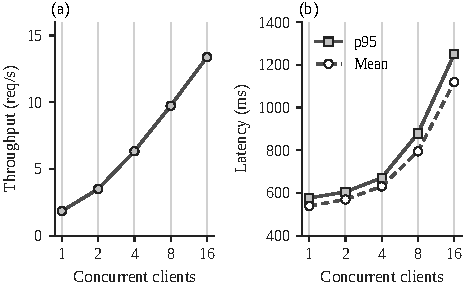
\includegraphics[width=\columnwidth]{imagens/fig6-calibration.pdf}
\caption{Measured RTX~5090 calibration (no TEE; 1{,}000 requests per point):
(a) throughput and (b) mean and p95 latency versus the number of concurrent
clients.}
\label{fig:scale}
\end{figure}

\begin{table}[t]
\caption{Physical CPU-thread ablation on the RTX 5090 benchmark.}
\label{tab:cpu-ablation}
\begin{tabularx}{\columnwidth}{c C C}
\toprule
\textbf{CPU threads} & \textbf{Mean latency (ms)} & \textbf{Success rate} \\
\midrule
16  & 1,099.05 & 100\% \\
32  & 1,114.15 & 100\% \\
64  & 1,117.82 & 100\% \\
192 & 1,118.40 & 100\% \\
\bottomrule
\end{tabularx}
\end{table}

\subsection{Trace-Driven Projection Method}

For backend $b$ and request $i$, the projected latency is
\begin{equation}
\label{eq:proj}
L^{\mathrm{TEE}}_{b,i} = L_i\,(1 + o_b) + a_i ,
\end{equation}
where $L_i$ is the measured latency of request $i$, $o_b$ is the relative
TEE overhead, and $a_i$ is the attestation cost charged to the request. The
overhead penalty of Eq.~(\ref{eq:op}) then becomes
$\mathrm{OP}_{b,i} = \min(1,\, o_b + a_i/L_i)$, and the CIS of every request
follows from Eq.~(\ref{eq:cis}).

The overhead $o_b$ is taken from the measurements summarized in
Table~\ref{tab:overheads}. For SGX and TDX, Chrapek \emph{et al.}
\cite{chrapek2025confidential} ran Llama-2-7B with 1{,}024 input and 128
output tokens, which matches the model and output length of our workload.
For SEV-SNP, no comparable LLM measurement was available, so we use the
transformer-inference (BERT-Large) results of Misono \emph{et al.}
\cite{misono2024cvm}, whose range reflects the effect of halt-polling
configuration. These studies run inference on the CPU, whereas our benchmark
runs on a GPU; applying their relative overhead to the whole end-to-end
latency is therefore conservative, because in a GPU deployment part of the
request time is spent outside the CPU-side protection. Each Monte Carlo draw
samples $o_b$ uniformly from its range, independently per backend.

\begin{table}[t]
\caption{Measured TEE overhead ranges used in the projection.}
\label{tab:overheads}
\begin{tabularx}{\columnwidth}{l c L}
\toprule
\textbf{Backend} & \textbf{Overhead} & \textbf{Source and workload} \\
\midrule
SGX     & 4.80--6.15\% & \cite{chrapek2025confidential}: Llama-2-7B, Gramine-SGX \\
TDX     & 5.51--10.68\% & \cite{chrapek2025confidential}: Llama-2-7B, TDX VM \\
SEV-SNP & 2.3--16\%     & \cite{misono2024cvm}: BERT-Large, SEV-SNP VM \\
\bottomrule
\end{tabularx}
\end{table}

Request arrival times are reconstructed from the measured elapsed time of each
round, so attestation freshness follows the real request rate of
14.12 requests/s. Each round opens a session with a full attestation, and a
full re-attestation is triggered whenever $\mathrm{AF}$ falls below
$\theta_{\text{att}}$. The plaintext and TLS-only references are scored with
the same Eq.~(\ref{eq:cis}). Neither has memory encryption or attestation
($\mathrm{PG} = \mathrm{AF} = 0$), and TLS record protection adds a negligible
cost against a 1.1\,s inference ($\mathrm{OP} \approx 0$). Their scores are
therefore $\mathrm{CIS} = 0.25$ for plaintext ($\mathrm{CS} = 0$) and
$\mathrm{CIS} = 0.2875$ for TLS-only ($\mathrm{CS} = 2/8$).

\subsection{Attestation Cost}
\label{subsec:att}

Table~\ref{tab:aa-perf} reports the attestation results. The 187\,ms full
attestation and 6.2\,ms cached check are conservative model inputs: Misono
\emph{et al.} \cite{misono2024cvm} measured the attestation primitives
themselves (quote or report generation and certificate and report
verification) at about 3.7\,ms on TDX and 9.9\,ms on SEV-SNP. The 187\,ms
value additionally covers collateral retrieval, network round trips, and
session setup. With $\lambda_a = 0.01$\,s$^{-1}$ and
$\theta_{\text{att}} = 0.90$, a full re-attestation is needed every
$-\ln(0.90)/0.01 = 10.54$\,s. At the measured request rate this occurs once
every $\approx 149$ requests: 8{,}048 full attestations over the 1.2 million
requests, a cache-hit rate of 99.33\%. The mean attestation cost is 7.41\,ms
per request, or 0.66\% of the measured latency, and the mean freshness score
is $\overline{\mathrm{AF}} = 0.949$. Attestation with freshness-aware caching
is therefore a minor cost compared with LLM inference.

\begin{table}[t]
\caption{Attestation over the 1.2 million projected requests (same model for
all backends).}
\label{tab:aa-perf}
\begin{tabularx}{\columnwidth}{L C}
\toprule
\textbf{Quantity} & \textbf{Value} \\
\midrule
Full attestation (ms; model input)        & 187 \\
Cached token check (ms; model input)      & 6.2 \\
Re-attestation interval (s)               & 10.54 \\
Full attestations                         & 8{,}048 \\
Cache-hit rate (\%)                       & 99.33 \\
Mean attestation cost per request (ms)    & 7.41 (0.66\%) \\
Mean freshness score $\overline{\mathrm{AF}}$ & 0.949 \\
\bottomrule
\end{tabularx}
\end{table}

\subsection{Projected Latency and Throughput}

Fig.~\ref{fig:perf} shows the projected mean latency of each backend against
the measured baseline. At the midpoint of the measured ranges, the projected
mean latency is 1{,}201\,ms for SGX (range 1{,}193--1{,}209\,ms),
1{,}231\,ms for TDX (1{,}201--1{,}260\,ms), and 1{,}242\,ms for SEV-SNP
(1{,}165--1{,}320\,ms), against 1{,}132\,ms measured without TEE. The
corresponding p95 latencies are 1{,}315, 1{,}347, and 1{,}360\,ms. Including
attestation, the effective overhead is 6.1\% (SGX), 8.8\% (TDX), and 9.8\%
(SEV-SNP). The projected throughput at 16 concurrent clients is 13.30, 12.98,
and 12.86 requests/s, against 14.12 measured. The SEV-SNP range is the widest
because its source measurements span configurations with and without halt
polling.

\begin{figure}[t]
\centering
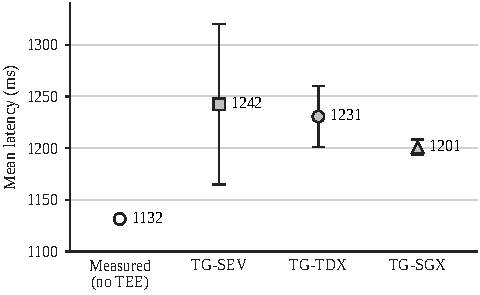
\includegraphics[width=\columnwidth]{imagens/fig4-latency.pdf}
\caption{Mean latency measured on the RTX~5090 without TEE (1.2 million
requests) and projected for each TwinGuard backend. Markers show the midpoint
of the measured overhead range (Table~\ref{tab:overheads}); whiskers show its
low and high ends. Projections include attestation.}
\label{fig:perf}
\end{figure}

\subsection{Confidential Inference Score}

Fig.~\ref{fig:security} compares the CIS of all configurations. All three
TwinGuard backends score far above the references, with 0.928 for SGX
[95\% interval 0.926--0.929], 0.921 for TDX [0.915--0.927], and 0.918 for
SEV-SNP [0.902--0.935], against 0.288 for TLS-only and 0.250 for plaintext.
This gap reflects the controls that the references lack, namely memory
encryption, attestation, and audit, rather than performance. All three
backends exceed the illustrative 0.90 threshold across their whole interval.

\begin{figure}[t]
\centering
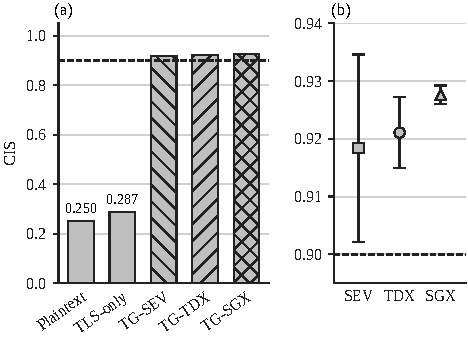
\includegraphics[width=\columnwidth]{imagens/fig5-cis.pdf}
\caption{CIS of the reference systems and the projected TwinGuard backends.
(a) Full scale; the references are computed with Eq.~(\ref{eq:cis}).
(b) TwinGuard backends: marker at the midpoint of the measured overhead range
and 95\% Monte Carlo interval. The dashed line marks the illustrative policy
threshold of 0.90.}
\label{fig:security}
\end{figure}

\subsection{Uncertainty of the Backend Ranking}

Because PG, AF, and CS are identical across backends under this projection,
the backend ranking depends only on the overhead term. It is therefore
insensitive to the CIS weights: any $\gamma > 0$ yields the same ordering,
and $\gamma = 0$ yields a tie. The relevant uncertainty is the TEE overhead
itself. Fig.~\ref{fig:cis-sensitivity} propagates it. SGX has the highest CIS
in 74.0\% of the draws, SEV-SNP in 23.8\%, and TDX in 2.2\%. The most frequent
ordering, SGX $>$ TDX $>$ SEV-SNP, occurs in 55.7\% of the draws. Under the
available measurements, SGX is the most likely to rank first, but no ordering
is certain: the wide SEV-SNP range overlaps both other backends, and its
outcome depends on the hypervisor configuration. This is a projection under
the cited measurements, not a ranking of physical deployments.

\begin{figure}[t]
\centering
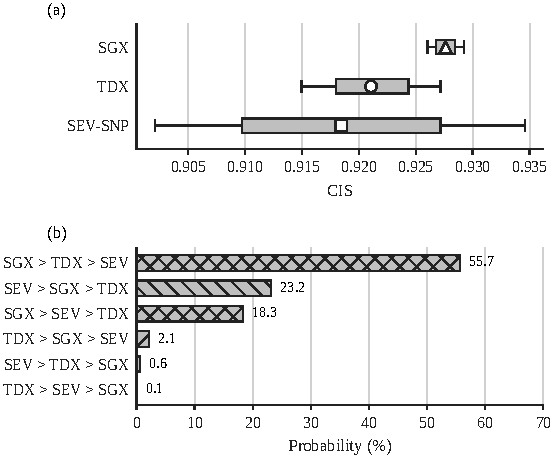
\includegraphics[width=\columnwidth]{imagens/fig7-uncertainty.pdf}
\caption{Monte Carlo uncertainty of the projection (4{,}000 draws over the
measured overhead ranges). (a) CIS distribution per backend: box from the 25th
to the 75th percentile, whiskers from the 2.5th to the 97.5th, marker at the
range midpoint. (b) Probability of each backend ranking.}
\label{fig:cis-sensitivity}
\end{figure}

% =============================================================================
\section{Discussion}
\label{sec:disc}
% =============================================================================

\subsection{Principal Findings}

The physical benchmark shows a stable, GPU-bound workload: 1.2 million
requests completed without failures, round means varied by less than 1\%, and
more than 16 host threads gave no benefit. Under the measured TEE overhead
ranges, confidentiality costs 6--10\% in latency at the range midpoints, about
70--110\,ms on a 1.1\,s request, and attestation with freshness-aware caching
adds less than 1\%.

The CIS separates protected from unprotected deployments clearly (about 0.92
against at most 0.29), but it cannot rank the three TEE backends with
certainty, because their ordering depends on overhead measurements that vary
with configuration, especially for SEV-SNP. The metric can therefore show
whether a deployment provides the intended controls at an acceptable cost.
Choosing a backend still requires measurements on the target platform.

\subsection{Limitations}

\textbf{Evaluation scope.} No TEE hardware was executed. The TEE results are
projections that combine measured per-request latencies with overhead ranges
reported by other studies \cite{chrapek2025confidential, misono2024cvm}.
These studies used CPU inference, different hardware, and, for SEV-SNP, a
different transformer model. The projection is therefore only as accurate as
those measurements and their transfer to a GPU-served workload, which we
expect to be conservative. Physical validation on TDX and SEV-SNP hosts,
ideally with a confidential GPU, is the main direction for future work
(Section~\ref{sec:conc}).

\textbf{Workload realism.} The prompts are random sequences from a 42-token pool
with fixed-length greedy decoding. This isolates serving performance from
content, but it does not reproduce the length and content distribution of real
traffic. The ten rounds replay the same dataset, so their agreement measures
stability; they are not independent samples.

\textbf{Hardware portability.} TwinGuard's hardware abstraction is
architectural; while the design requires no LLM-stack modifications across
TEE backends, full cross-backend operational equivalence has not been validated on
hardware. Differences
in memory models, attestation APIs (DCAP vs.\ AMD-SP/KDS), and secure
I/O paths across SGX, TDX, and SEV-SNP may require backend-specific
adaptation during deployment.

\textbf{Side-channel residual risk.} TwinGuard does not eliminate all
side-channel risks, particularly for SGX where cache-timing and page-fault
channels remain exploitable \cite{brasser2017software, xu2015controlled}.
Users in high-threat environments should evaluate a properly attested TEE deployment and apply additional mitigations; however, our results do not support
choosing between TDX and SEV-SNP for physical deployment.

\textbf{GPU memory security.} The framework is designed to integrate CPU-side TEE protections. Extending this trust boundary to the GPU depends on
dedicated confidential-computing capabilities. In the RTX 5090 reference benchmark, the GPU-resident model weights, activations, and associated data paths
are outside the CPU-side TEE boundary and are not evaluated by this benchmark.
Current GPU-TEE integration
approaches (e.g., NVIDIA H100 Confidential Computing mode) are nascent and not
yet standardized, and future work should evaluate TwinGuard in conjunction with
GPU-side confidential computing.

\textbf{CIS weights and threshold.} The reference weights
$(\alpha,\beta,\gamma,\delta)=(0.35,0.25,0.25,0.15)$ are security-centric policy choices. Because PG, AF, and CS are equal across backends in this
projection, the backend ordering does not depend on the weights, as long as
$\gamma>0$ (an offline sweep over 176{,}851 weight vectors on a 0.01 simplex
grid confirms this; the script \texttt{cis\_weight\_sensitivity.py} is in the public repository). The weights change the absolute scores and the distance to the threshold. The 0.90 threshold is a
policy value and not a regulatory criterion: with the design-level coverage
$\mathrm{CS}=0.9375$, the bound of Eq.~(\ref{eq:threshold}) is
$\mathrm{CIS}\ge 0.893$, so a deployment at the edge of the stated
freshness, privacy, and overhead conditions could fall slightly below it.

\textbf{DP accuracy impact.} The differential privacy mechanism introduces
a quality-utility tradeoff. We did not measure LLM output quality for
$\epsilon < 1.0$; differentially private
fine-tuning results \cite{yu2022differentially} suggest that moderate utility
cost is possible at $\epsilon \approx 6$--$7$, but this concerns training,
not inference-time perturbation, and has not been verified for TwinGuard.

\textbf{Privacy and attack evaluation.} This study does not report the original perplexity, utility, membership-inference, model-extraction, or model-inversion
experiments; the attack and utility results cited in Section~\ref{sec:bg}
come from other systems.

\textbf{Technical-mapping gap.} The $6.2$~pp gap in the selected
technical-control mappings arises from data minimization decisions that cannot be fully
automated without domain-specific policy annotations. Future work should
address policy-as-code integration.

\subsection{Threats to Validity}

\textbf{Internal validity.} The projected TEE latencies and CIS values depend
on three groups of inputs: the measured overhead ranges, the attestation
latencies (187\,ms and 6.2\,ms), and CIS weights. The measured latencies and request timing originate from the physical traces. Errors
in the overhead measurements propagate directly to the projections, which is
why we report them as ranges and propagate them using the Monte Carlo method.

\textbf{External validity.} The results apply to transformer-based LLMs in the
7B parameter range. Larger models (70B, 405B) may exhibit different overhead profiles owing to memory bandwidth constraints.

\textbf{Construct validity.} CIS is defined by the authors and reflects our
operationalization of the GDPR and HIPAA requirements; other
operationalizations may yield different rankings. It has not been validated
against independent compliance audits or membership-inference measurements,
and its weights and 0.90 threshold are a security-centric policy choice
(Section~\ref{subsec:cis}). CIS is not a recognized regulatory standard and
does not replace a formal compliance audit.

\textbf{Data sovereignty.} GDPR Chapter~V (Arts.\ 44--49) governs
international transfers of personal data. TEE-based processing does not satisfy data residency or transfer adequacy requirements; a
TwinGuard deployment must still ensure that inference is performed within
the appropriate jurisdiction or under a valid transfer mechanism
(adequacy decision, SCCs, or BCRs). TwinGuard's technical controls do not
address this requirement.

% =============================================================================
\section{Conclusion and Future Work}
\label{sec:conc}
% =============================================================================

TwinGuard organizes confidential LLM inference around three agents: one that
manages vendor attestation chains with freshness-aware caching, one that runs
memory-encrypted inference with optional output perturbation, and one that
keeps a tamper-evident Merkle ledger mapped to the selected GDPR and HIPAA controls. The CIS combines these properties with the cost of protection in a
single score.

Projected over 1.2 million requests measured on an RTX~5090, confidential
inference costs 6--10\% in latency at the midpoints of the published TEE
overhead ranges, and freshness-aware attestation adds 0.66\%. For a
regulated deployment, the cost of protection is therefore small next to the
inference itself. The available measurements do not settle which backend is
best: SGX ranks first in 74\% of the Monte Carlo draws, and the SEV-SNP range
overlaps both others. The most important next step is to measure TwinGuard
directly on TEE hardware.

Future work will address five directions:

\begin{enumerate}
\item \textbf{Physical hardware validation.} Deploying and benchmarking
TwinGuard on Intel TDX and AMD SEV-SNP hosts, ideally with a confidential
GPU, to replace the projected overheads with direct measurements and confirm
cross-backend portability.

\item \textbf{Large-model support.} Extending the chunk-based memory
architecture to 70B and 405B parameter models using pipelined decryption
and NVMe-level encryption offload.

\item \textbf{Multi-party inference.} Enabling federated inference across
multiple TEE-protected nodes, combining TwinGuard with verifiable secret
sharing to support distributed LLM deployments.

\item \textbf{Adaptive DP budgeting.} Integrating the R\'enyi DP accountant
\cite{mironov2017renyi} for tighter privacy accounting across heterogeneous
query sequences.

\item \textbf{Policy-as-code compliance and CIS external validation.}
Developing a domain-specific language for regulatory policy annotation that
the Audit Agent can evaluate at runtime, closing the residual compliance
coverage gap. Concurrently, correlating CIS measurements with independently
assessed compliance audits and empirical membership-inference attack success
rates to establish external validity for the metric; and integrating TwinGuard
with GPU-TEE mechanisms (e.g., NVIDIA H100 Confidential Computing mode
\cite{nvidia2023cc}) to extend the TEE trust boundary to GPU-resident
weights and activations.
\end{enumerate}

% =============================================================================
\section*{Acknowledgment}
% =============================================================================

The authors acknowledge the use of Claude (Anthropic) as a language model
assistant during the preparation of this manuscript, specifically for
literature synthesis, language revision, and structural organization in the
Introduction, framework, evaluation, and discussion sections. The tool was
not used to generate experimental data, results, figures, references, or
technical claims. All scientific content, methodological decisions, data
interpretation, and intellectual contributions remain the sole responsibility
of the human authors.

This research was partially supported by the Funda\c{c}\~ao Amaz\^onia de
Amparo a Estudos e Pesquisas do Par\'a (FAPESPA), the Centro de Pesquisa e
Desenvolvimento em Tecnologias Digitais para Informa\c{c}\~ao e
Comunica\c{c}\~ao (PRODEPA), and SEC365 Cybersecurity Solutions. The authors
also thank the Laborat\'orio de Intelig\^encia Computacional e Aprendizado
(LICA), the Centro de Compet\^encia em Aplica\c{c}\~oes e Dados da
Intelig\^encia Artificial (CCAD-IA), the Rede Nacional de Ensino e Pesquisa
(RNP), and the Instituto Nacional de Ci\^encia e Tecnologia em Intelig\^encia
Artificial na Amaz\^onia (INCT iAmazonia) for providing computational
infrastructure and research collaboration support.
\section*{Data Availability}
The per-request baseline traces, workload and environment manifests, SHA-256
checksums, projection code, and figure-generation scripts that support the
findings of this study are openly available at
\url{https://github.com/ufxa/tee-llm-inference}. No physical TEE measurements are included; all TEE
results are trace-driven projections.

% =============================================================================
\bibliographystyle{IEEEtran}
\bibliography{references}
% =============================================================================

\begingroup
\renewcommand{\addcontentsline}[3]{}

\begin{IEEEbiography}[{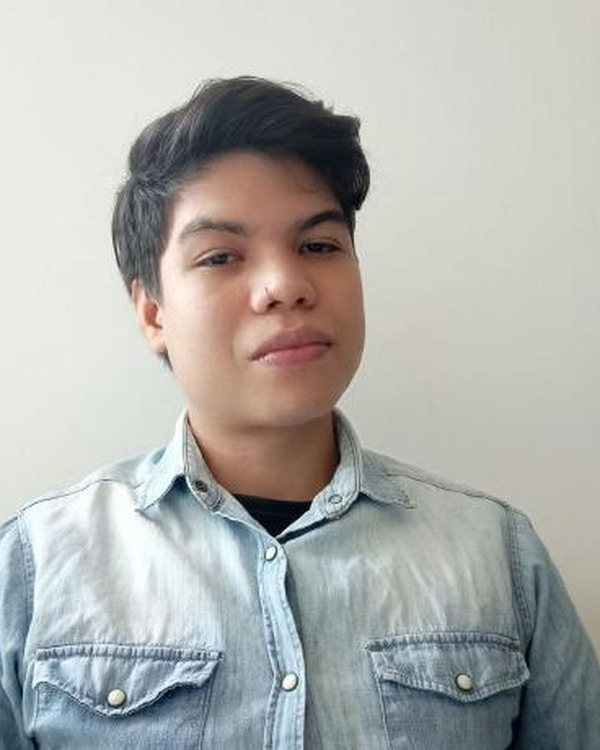
\includegraphics[width=1in,height=1.25in,clip,keepaspectratio]{imagens/bio-barbosa.jpg}}]{Carlos Lucas Vieira Barbosa}
received the B.S. degree in telecommunications engineering from the Federal
University of Par\'a (UFPA), Bel\'em, Brazil, in 2025. Barbosa's research
interests include cybersecurity, confidential computing, and
privacy-preserving artificial intelligence.
\end{IEEEbiography}

\begin{IEEEbiography}[{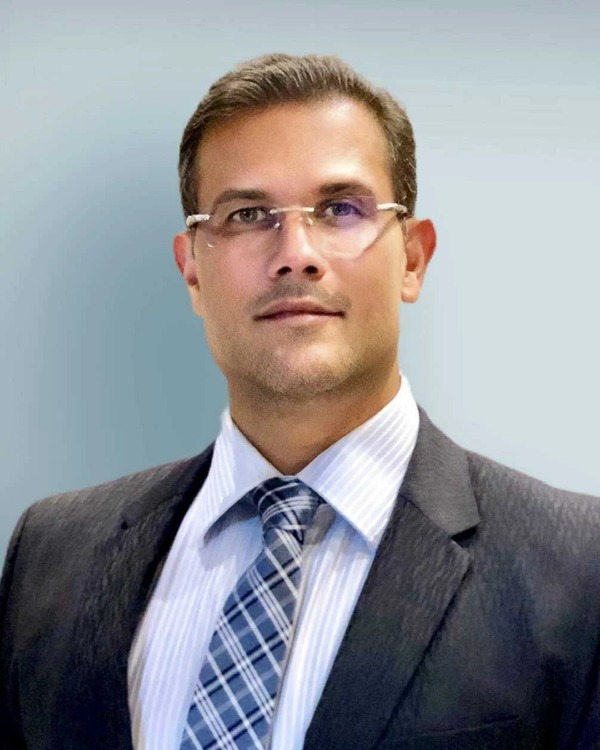
\includegraphics[width=1in,height=1.25in,clip,keepaspectratio]{imagens/bio-souza.jpg}}]{Jos\'e de Souza Junior}
is a lawyer, a researcher at the University of Bras\'ilia (UnB), Bras\'ilia,
Brazil, and a consultant in cybersecurity and artificial intelligence, with
extensive experience in risk prevention and mitigation in both the private and
public sectors. Souza Junior is currently pursuing the D.B.A. degree at the University
of Bordeaux, France. Souza Junior received the master's degree in law and
economic management, with specialization in finance, from Sorbonne
Universit\'e, Paris, France, a postgraduate degree in business management from
Funda\c{c}\~ao Dom Cabral, the LL.M. degree in business law from IBMEC, and
specializations in public law (Dam\'asio Educacional) and in civil law and
civil procedure (UNIVEM). Souza Junior also holds an MBA in cybersecurity and
digital management from FIA and completed cybersecurity programs at Harvard
University and at MIT Sloan Executive Education.
\end{IEEEbiography}

\begin{IEEEbiography}[{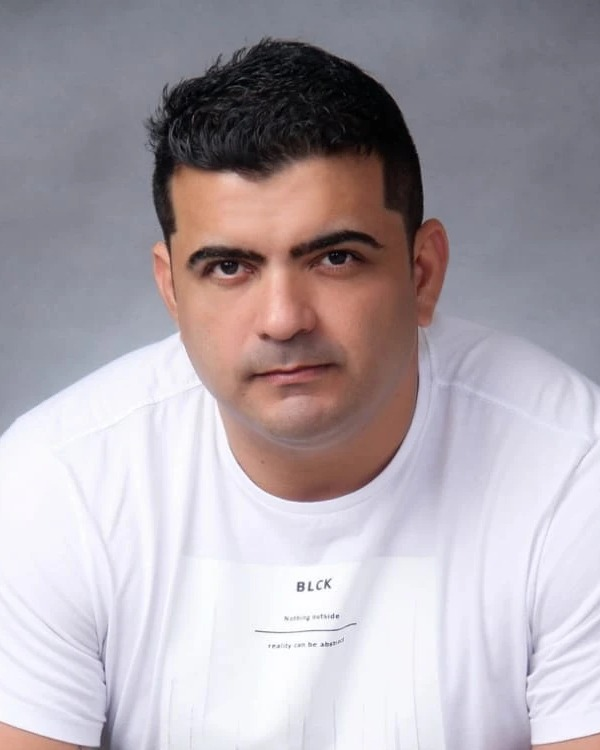
\includegraphics[width=1in,height=1.25in,clip,keepaspectratio]{imagens/bio-costa.jpg}}]{Allan Douglas Costa}
received the M.S. and Ph.D. degrees in computer science, holds two
postdoctoral appointments and three specializations, and is a Permanent
Professor at the Federal Rural University of the Amazon (UFRA), Bel\'em,
Brazil. Costa has more than 25 years of experience in the technology sector,
having served as Chief Technology Officer, information security consultant,
digital forensics expert, senior security analyst, security officer, and leader
of security intelligence and content security teams, and has taught at UNAMA,
IFPA, CESUPA, Est\'acio/IESAM, FAPAN, Faculdade Integrada Ipiranga, and FAPEN.
Costa founded and leads the research group Centro Aplicado de Intelig\^encia em
Ciberseguran\c{c}a (CAIC/CNPq) and is a permanent member of the N\'ucleo de
Pesquisas em Computa\c{c}\~ao Aplicada (CNPq/UFRA). Costa holds the CCISO,
CISM, CISO, CRISC, CEH, CHFI, CASP+, Security+, CySA+, CPENT, ISFS 27001, PMP,
PDPP, CSA, and CNSS certifications, is a member of the IEEE and of the
Brazilian Computer Society (SBC), serves as a reviewer for IEEE Access and Science Publishing Group, and has
edited two books.
\end{IEEEbiography}

\endgroup

\EOD

\end{document}
